\chapter{Usability Testing}
\label{sec:Usabilitytesting}
This section will explain what usability testing is, and what we did during our project relating to usability testing.

\section{What is usability testing}
Usability testing is a way to test your system on users, using the interaction design of the system. Usually this entails setting up 
a few tasks for a user, giving the user access to the system and seeing how well the user is able to solve the tasks given in the test
with the system provided. The usability testing focuses on the main functionality rather than on the details. 

\section{How to do usability testing}
The test usually starts with the tester explaining for the user the different parts of the systems being used, and that it's the system being
tested, not the user. The tester also explains that this means the user can't do anything wrong, if there is something the user doesn't 
understand, that is fine. The tester observe what the user finds hard, or can't do at all, and notes this down as things that might have
to be changed on the system. 

At last, the user is given an evaluation form of the system, typically a SUS-form (System Usability Scale), and time to talk about
how well they felt the system helped them solve the tasks given. %Add reference to SUS?

\section{Usability testing in our project}
Our project largely implements user interraction, and usability testing plays a key role in getting a good result, since so much
of the project is centered around the user interface. We started the project with an early paper prototype test, to get some feedback on the ideas
we got after the workshop we did with the interaction design group. After this we worked for some time on implementing the system, before we late in
the project did a full usability test using the hallway method, testing our system on children to see if it helped them take their medicine, and seeing
if there was some bugs or things we could implement better.

\subsection{Paper prototype test}
\label{sec:paperprototypetest}
In the early stages of development, it might be useful to do a paper prototype test. This test is done by making a prototype of the user interface on paper, 
and having one person (the "computer") change between the different paper screens based on what the user being tested clicks on. 

We did some early paper prototype testing in our project, on the 4th of September. After our workshop we had made some screen layout mockups, see figure \ref{fig:paperprototype}, 
and we wanted to test how user friendly these were.

\begin{figure}
	%\vspace{-4cm}
	%\hspace{4cm}
	\center
		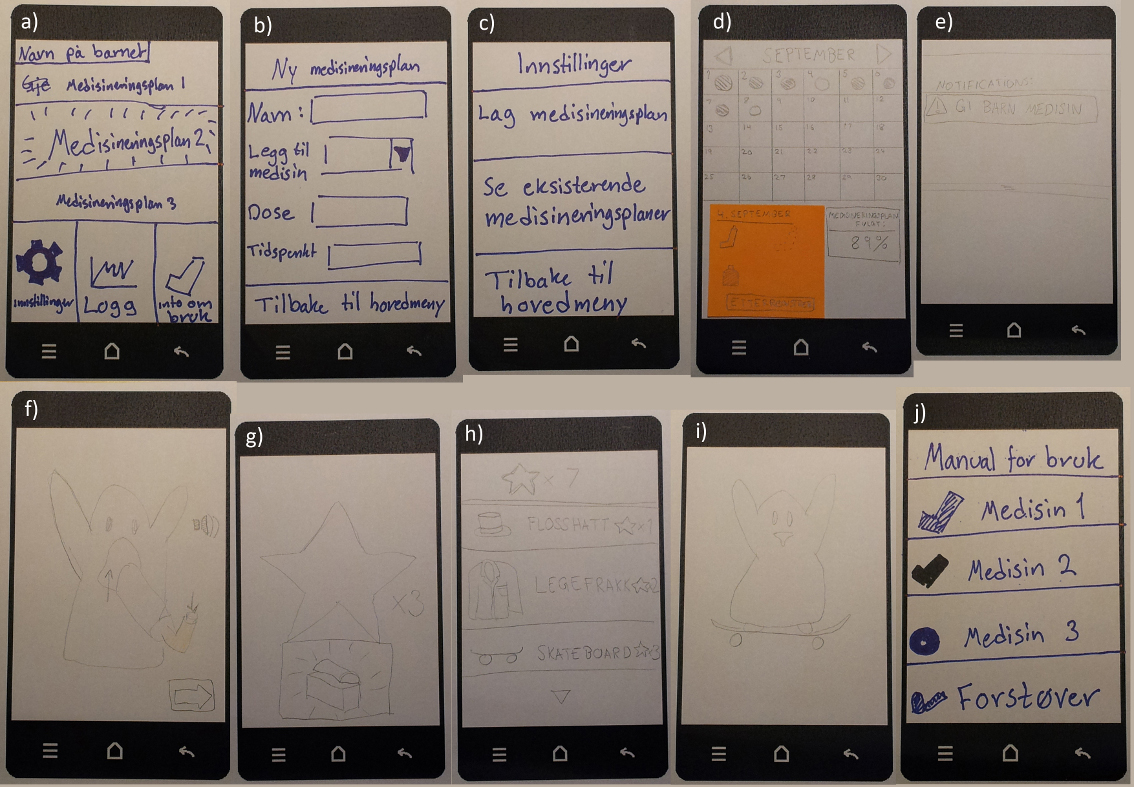
\includegraphics[width=0.8\paperheight, angle=90]{Pictures/PaperprototypeScaled}

	\caption[Paper prototype]{The screens of the paper prototype: a) The GAPP mainscreen. 

								b) GAPP new medication screen.
								c) GAPP settings screen
								d) GAPP log screen.
								e) Notification on phone
								f) One of the CAPP distraction screens.
								g) The CAPP reward screen
								h) CAPP shop screen
								i) CAPP avatar screen, after buying skateboard in the shop
								j) the GAPP manual screen}
	\label{fig:paperprototype}
\end{figure}

The test was done with the expert review method. We had a person from NAAF come for the test, to solve the tasks with the system we provided. We chose to do the expert
review mainly because our funder was interested in seeing how the project was proceeding. NAAF is also the main provider of information such as instructions and 
how the medical plans looks, so having one of them see the system was helpful, as we at this point was uncertain about alot of these things.

From the development group, Eirik and Aleks attended the test. Eirik played the part of the computer, while Aleks introduced the test, explained the system and handled
any other talking that needed to be done.\\
The preconditions we assumed to be present for the CAPP was:
\begin{itemize}
	\item A paper prototype with the correct screens.
	\item Basic knowledge of Android devices in the user being tested.
	\item An active notification for taking medicine on the android device.
\end{itemize}
for GAPP these precondition were:
\begin{itemize}
	\item A paper prototype with the correct screens.
	\item Basic knowledge of android devices in the user being tested.
	\item The correct medication plans and medicines registered in the system.
\end{itemize}

We had prepared a set of tasks for each of our two android applications, CAPP and GAPP. We did not have a functional application for the karotz at this point, and it was difficult to
test this with a paper prototype, so we chose to leave that part out of this test. The cases can be seen in table \ref{tab:capptasks} and table \ref{tab:gapptasks}.

\begin{table}[h]
	\begin{center}
		\begin{tabular}{|p{1.0cm}|p{10.0cm}|}
			\hline
			\bf{Task} & \bf{Description}\\
			\hline
			\bf{1} & There is an active notification for medication on the phone, follow the instructions given by the android device.\\
			\bf{2} & Go to the shop in CAPP and buy a skateboard for the avatar.\\
			\hline
		\end{tabular}
	\end{center}
	\caption{The tasks for CAPP}
	\label{tab:capptasks}
\end{table}

\begin{table}[h]
	\begin{center}
		\begin{tabular}{|p{1.0cm}|p{10.0cm}|}
			\hline
			\bf{Task} & \bf{Description}\\
			\hline
			\bf{1} & Open GAPP.\\
			\bf{2} & Register use of "Medisin 1" on 4th of september.\\
			\bf{3} & Check for more iformation on correct usage of "Medisin 2".\\
			\hline
		\end{tabular}
	\end{center}
	\caption{The tasks for GAPP}
	\label{tab:gapptasks}
\end{table}

This test gave us some strong feedback on what parts of the system worked well, and what didn't make sense at all. We also sat down and had an interview with
the test person after the test regarding the best way to present the information we would get from NAAF.
Some of the problems the test person had might be credited to her being inexperienced with android devices, but we noted down these problems aswell.
 In short the paper prototype test gave us the following results:

\begin{itemize}
	\item Having the reminder as a notification is insufficient. The test person had trouble noticing it even though she was told it would be there.
	\item CAPP have to inform how many times you should press the medicine during medication.
	\item The rewardscreen in CAPP is not intuitive enough.
	\item The main menu in GAPP needs a complete rework, the menu system was not easy to understand.
	\item The Log have to be clearer on how to register medicines, and which medicines is already registered.
	\item There is no back button in the application. This is a problem with android experience, and we didn't implement a back button in the end.
	\item The Information about correct use of medicines was not easily accessible.
\end{itemize} 
The paper prototype led to a major overhaul of the user interface.

\subsection{Usability testing of the distraction}
\label{sec:usabilitytestonchildren}
Since our system is targeted towards children it was important to test the system properly on children, to see if the effects where as we hoped for. This was difficult to do early in the project since the children could not be expected to deal with paper prototypes, as they were as young as three years old. Because we had to create our system from scratch, it took a long time to get something robust enough to test, there was a long process of unit and integration testing going into making the communication between two Android applications and one Karotz application.

This led to a late usability test, held on 30th of October 2012. At this point we had a working version of the system. 

The preconditions for the test were:
\begin{itemize}
	\item Working version of CAPP and the karotz application.
	\item The child in the database is registered to the correct health state.
	\item Child and parent present. The parent should be familiar with giving asthma medications\footnote{The application gives information about this, but it is not what is being tested}.
	\item Wireless wpa2 secured connection for the karotz.
\end{itemize}

The test started with some basic introduction, done informally. Trying to run a standard usability test on already shy children was not optimal, so we explained to the parents, and let them tell the children what was going to happen. After giving an introduction, we registered a new medication plan in the database, with alarm set for one or two minute in the future. We had to register it this way to make sure the reward system and log updated properly in response to the treatment.\\ 
The test scenario we wanted for CAPP was as follows:
\begin{itemize}
	\item The Android device receives an alarm. The parent hands the phone to the child.
	\item After finding the correct medicine, based on the picture on the alarmscreen, the child starts the distraction sequence.
	\item The child follows the instructions given during the distraction sequence, and does as the karotz on the screen.
	\item The child, helped where necessary by their parent, successfully takes their medicine.
	\item After the distraction finishes, the child is done with their treatment, and receives the reward in the application.
\end{itemize}
For the karotz application, this scenario plays out a little bit differently:
\begin{itemize}
	\item The robot gives a notification.
	\item The child follows the instructions to turn off the notification and ready the distraction.
	\item After fetching the parent, the child is given the yellow nanoz by their parent, and holds the yellow nanoz close to the karotz' nose to start the distraction sequence.
	\item The child and parent follows the instructions given during the distraction sequence, which helps the child successfully take their medicine.
	\item After the distraction sequence finishes the child uses the green nanoz to collect their reward from the karotz.
\end{itemize}

Before the test we had already discovered that the Karotz was quite selective in it's internet connections security protocols, and it could not connect to for example the "eduroam"
network found at the university. The previous day we tried using a wireless router of our own and connecting this to one of the internet cables at a computer lab at NTNU. This apporach had worked fine, but we wanted to make sure it was up and running by the time the test were to start. We found out this would not
work with the internet at NSEPs usability lab, and we only barely got it up and running by using a smartphone to set up a wireless hotspot for the Karotz. A description of the problems are reported, for future development in \ref{sec:Improvements}. 

The test was done using the hallway method, meaning we let users who had little or no prior knowledge of the system test it. Some pictures from the tests can be seen below:
\begin{figure}
	\centering
		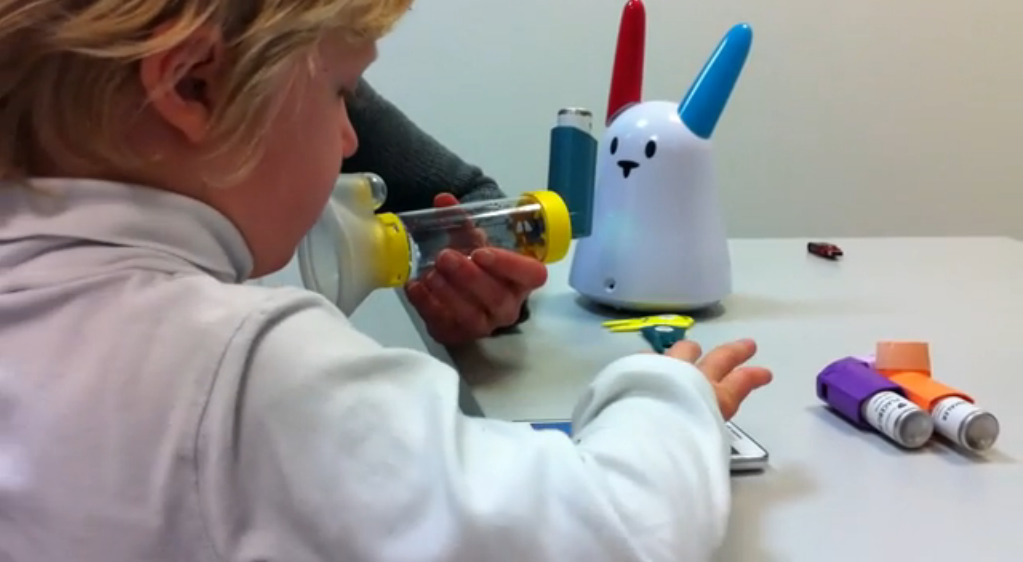
\includegraphics[width=\linewidth]{Pictures/usabilitytestCAPP}
	\caption[Usability test CAPP distraction]{Child taking their medicine while following the CAPP distraction sequence. Photo: Elin Høien}
	\label{fig:cappdistraction}
\end{figure}

\begin{figure}
	\centering
		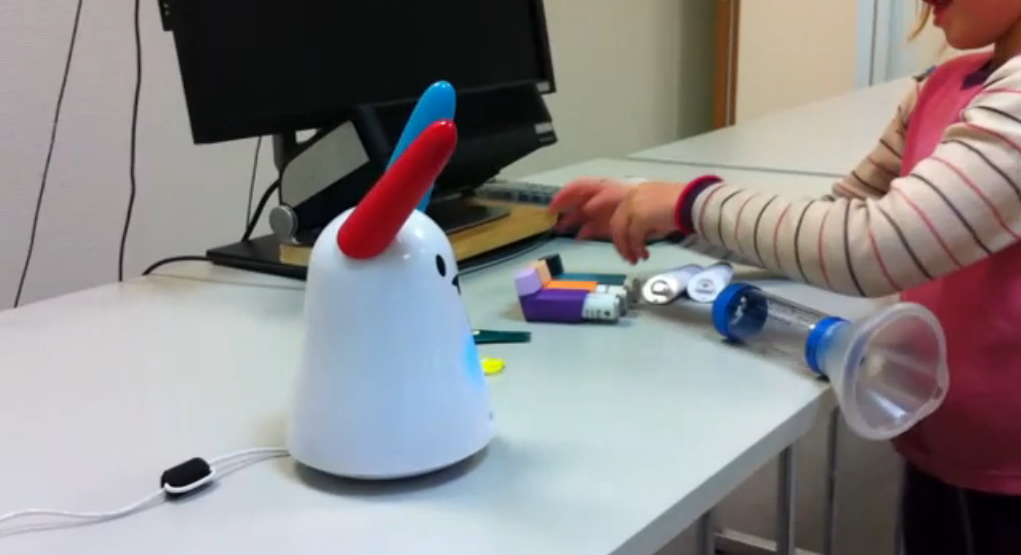
\includegraphics[width=\linewidth]{Pictures/usabilitytestkarotz}
	\caption[Usability test Karotz distraction]{Child taking their medicine while following the Karotz distraction sequence. Photo: Elin Høien}
	\label{fig:karotzdistraction}
\end{figure}

\begin{figure}
	\centering
		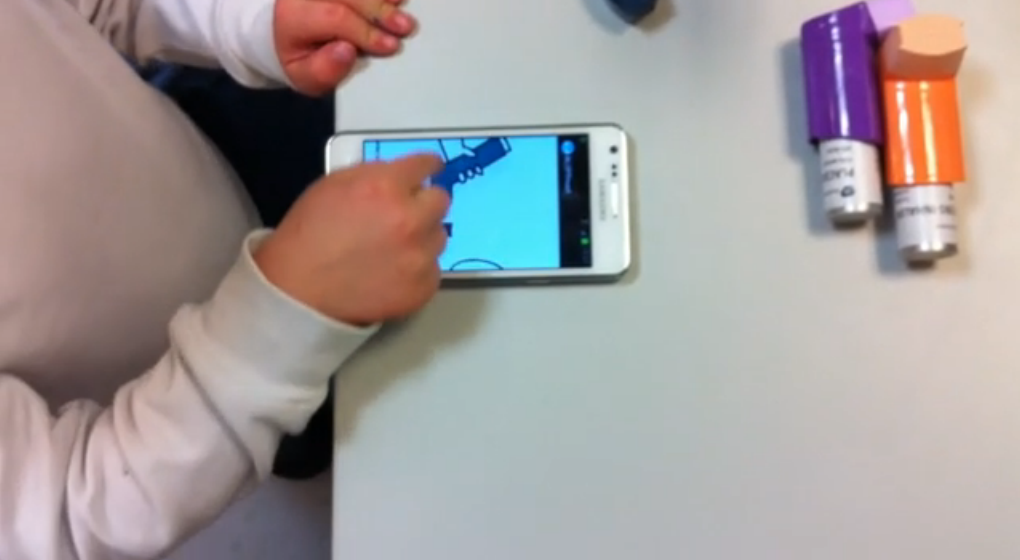
\includegraphics[width=0.4\paperheight, angle=90]{Pictures/usabilitytestinstructions}
	\caption[Usability test CAPP instructions]{Child distributing medicine to the karotz while looking at the instruction manual in CAPP. Photo: Elin Høien}
	\label{fig:cappinstructions}
\end{figure}

After the internet connection for the karotz was secured, the test ran without other big problems. We observed the following during the tests: the children
managed to follow the instructions given by both CAPP and the Karotz application. Some of the children were reluctant to actually take medicine, but they were eager to see what happened
next on the application, and we hope this will motivate them to take their medicine, even for the children who does not really want to take their medicine. We feared that our reward system would be too simple and
therefore not rewarding enough, but the children who tested the system seemed very interested in it, even though it was just points you gather in the form of stars. One of the children started comparing the amount after each treatment and ran the treatment many times in order to get the most
points possible. (We later implemented a time check, blocking the user from doing several treatments in a row).
We noted that the children were quick to become friendly with the Karotz, especially when it started talking.

We also uncovered quite a few bugs and parts that needed to be redone. For CAPP, the most important of these was:
\begin{itemize}
	\item The alarms were not deleted properly. Since we update them regularly to ensure they're fired properly, this resulted in alarms firing at the same time, resulting in a lot of noise, aswell as
		untimely fired alarms (which should have been moved).
	\item The alarm sound did not turn off when the distraction sequence ended, or when the "stop alarm" button was pushed. 
	\item After the distraction sequence the children did not understand that the chest was interactable, since the rest of the sequence were spoken, and this was not. However, after seeing the chest
		in the main menu, they understood that they could click it.
	\item If the user pressed the screen multiple times, this registered as multiple clicks, and parts of the distraction sequence was skipped. This happened frequently, as the children pressed again
		because of the delay between the first click register, until the screen updated.
	\item Part of the instructions had been left out in the distraction sequence, namely the one about rinsing your mouth after taking the medication.
	\item The instruction about pressing the medicine once, before breathing 10 times, were not clear. One of the children pressed the medicine 10 times.
\end{itemize}
There were also bugs and problems related to the Karotz, aside from the big issue with network connection:
\begin{itemize}
	\item The Karotz instructed the user to hold the Nanoz close to its belly, which is incorrect. For the Nanoz to register, they must be held close to the nose. 
	\item The distraction sequence never says to attach the medicine to the chamber.
	\item Holding the Nanoz close for too long makes the Karotz skip instructions. 
	\item As with CAPP, it was not clear that they had to press the medication once before inhaling 10 times.
\end{itemize}